A ergodicidade da medida produto
tem como conseqüência que, quase certamente, existe um aglomerado infinito quando
$\tep>0$. 

De fato, o evento de que existe um aglomerado infinito
($\cup_{x\in\zzd}\{|C_x|=\infty\}$) é invariante por translação e portanto
trivial sob $\p$. (O que decorre também deste evento ser caudal e da Lei
0-1 de Kolmogorov.)

Neste capítulo, a ergodicidade será 
explorada para estabelecer um dos aspectos mais interessantes desta fase, o fato de que
o aglomerado infinito é único (quase certamente).

Vamos definir por $\eta$ a variável aleatória que conta o número de aglomerados infinitos distintos
de uma configuração de $\Om$.  
$\eta$ é invariante por translação (pois translações das configurações de $\Om$ não alteram 
o número de aglomerados infinitos delas) e as medidas $\p$ são ergódicas, por serem  
produto. Portanto, por uma conhecida lei 0-1, $\eta$ é constante quase certamente. Em 
princípio,
$\eta$ pode assumir qualquer valor inteiro, desde $0$ até $\infty$.
O  resultado principal deste capítulo exclui $\eta\geq2$.

\vs

\bte
\label{teo:uni}
Qualquer que seja $p\in[0,1]$,
\beq
\p(\eta=0)=1
\eeq
ou
\beq
\p(\eta=1)=1.
\eeq
\ete

\vs

O Teorema~\ref{teo:uni} é provado por meio das seguintes proposições, devidas
respectivamente
a Newman e Schulman~\cite{kn:NS} e Aizenman, Kesten e 
Newman~\cite{kn:AKN}. A primeira, exclui $2\leq\eta<\infty$.  
A segunda exclui $\eta\geq3$. (Infelizmente, não se pode
incluir $\infty$ na primeira ou $2$ na segunda.)

\vs

\bpro
\label{prop:uni1}
Qualquer que seja $p\in[0,1]$,
\beq
\p(\eta=0)=1
\eeq
ou
\beq
\p(\eta=1)=1
\eeq
ou
\beq
\p(\eta=\infty)=1.
\eeq
\epro

\vs

\noindent {\bf Prova}

Seja $k_p$ a constante tal que $\p(\eta=\kp)=1$. Suponha que $1\leq\kp<\infty$. Vamos 
mostrar que disto se segue que $\p(\eta=1)>0$, o que implica pela trivialidade de $\eta$ que $\kp=1$.

De fato, denotando por $\qn$ o cubo de lado $2n+1$ centrado na origem., considere o 
evento 
\beq
\an=\{\mbox{todos os aglomerados infinitos intersectam $\qn$}\}.
\eeq
Note que $\an$ depende da configuração de elos apenas da fronteira de $\qn$ para fora.
Como $\kp<\infty$,  
\beq
\lim_{n\to\infty}\p(\an,\eta=\kp)=\p(\eta=\kp)=1.
\eeq


Seja $n_0$ tal que $\p(\anu)>0$ e considere o evento 
\beq
\bnu=\{\mbox{todos os elos interiores de $\qnu$ estão abertos}\}.
\eeq
Note que $\bnu$ depende apenas dos elos interiores a $\qnu$ e logo
é independente de $\anu$.

Finalmente, o evento de que $\eta=1$ contem $\anu\cap\bnu$.
Concluimos da discussão acima que
\beq
\p(\eta=1)\geq\p(\anu\cap\bnu)=\p(\anu)\p(\bnu)>0. \bo
\eeq

\vs

\bpro
\label{prop:uni2}
Qualquer que seja $p\in[0,1]$,
\beq
\p(\eta\geq3)=0.
\eeq
\epro

\vs

Deste resultado apresentaremos uma prova
diferente da original de Aizenman, Kesten e Newman, 
mais simples e geral, devida a Burton e Keane \cite{kn:BK}.
Ela se vale do argumento geométrico esboçado a seguir.

A ocorrência de três aglomerados infinitos disjuntos (e a ergodicidade de $\p$) tem como 
conseqüência a existência de uma densidade de {\em pontos triplos especiais}, isto é, sítios 
ligados por elos disjuntos a três aglomerados infinitos, que seriam disjuntos ao
se remover os elos incidentes àqueles sítios. Mas um lema sobre grafos
(que será enunciado abaixo como exercício) mostra que dentro de um cubo podem existir um número de pontos 
triplos especiais apenas da ordem da área da fronteira do cubo. Da contradição segue o 
resultado da proposição.

Agora enunciamos o lema sobre grafos, em forma de exercício para o leitor.

\vs

{\bf Exercício}

Seja G um grafo conexo com conjunto de sítios S e conjunto de elos E. Um sítio
$x$ em S ser\' a chamado um {\em ponto triplo} para G se

\begin{itemize}
\item[i)] existirem apenas três elos de E tocando $x$ e
\item[ii)] o grafo G$\backslash$\{$x$\}, em que $x$ é removido de S e os três
elos tocando em $x$ são removidos de E, tem exatamente três componentes
conexos. (Denotaremos os conjuntos de sítios destes três componentes
$E_1(x),E_2(x),E_3(x)$ e os chamaremos de ramos. Veja Figura~\ref{fig:pt}.)
\end{itemize}


\bef
%\input pt
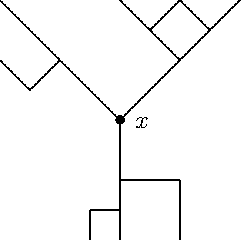
\includegraphics{pt}
\caption{$x$ é um ponto triplo}
\label{fig:pt}
\eef


a. Suponha que G seja um grafo conexo e que $x_1,x_2,\ldots,x_n$ sejam
pontos triplos distintos para G. Mostre que para algum i dois dos três
ramos em $x_i$, digamos $E_2(x_i)$ e $E_3(x_i)$ não contêm nenhum dos
outros pontos triplos ($\{x_1,\ldots,x_n\}\backslash\{x_i\}$).[Sugestão:
indução em n]

b. Considere o grafo $\mbox{G}'$ obtido de G e $x_1,\ldots,x_n$ do item anterior
remo\-ven\-do-se todos os sítios de $E_3(x_i)$ e todos os elos tocando estes
sítios. Mostre que $\{x_1,\ldots,x_n\}\backslash\{x_i\}$ são pontos triplos
para $\mbox{G}'$.

c. Suponha que G seja um grafo conexo e que $x_1,\ldots,x_n$ sejam pontos triplos
distintos de G. Entre os 3n ramos,
$$E_1(x_1),E_2(x_1),E_3(x_1),E_1(x_2),\ldots,E_3(x_n),$$
mostre que se pode achar pelo menos n+2 ramos {\em disjuntos}.

\vs

\noindent {\bf Prova da Proposição~\ref{prop:uni2}}

Suponha que $\p(\eta\geq3)>0$. Vamos procurar uma contradição.

Seja o evento
\beqnn
\fn\=\{\mbox{pelo menos três aglomerados infinitos abertos distintos}\\
&&\mbox{atingem $\qnm$}\}.
\eeqnn

Note que $\fn\uparrow\{\eta\geq3\}$ quando $n\uparrow\infty$, logo
existe $n_0$ tal que $\p(\fnu)>0$. Dados $\y$ três pontos distintos
no interior das faces de $\partial\qnu$, seja o evento
\beqnn
\fnu(\y)\=\{\y\,\,\mbox{pertencem a aglomerados infinitos distintos}\\
&&\mbox{usando apenas elos exteriores a $\qnu$}
\footnotemark\}.
\eeqnn
\footnotetext{exclui elos com pelo menos uma extremidade em $\qnm$}
Como $\fnu\subset\bigcup_{\y}\fnu(\y)$, temos que
\beq
\p(\fnu(\y))>0
\eeq
para algum $\y$. Dados estes $\y$, seja $x=x(\y)$ um ponto do interior
de $\qnu$ com a propriedade de que há três caminhos de elos disjuntos
no interior $\qnu$\footnote[2]{$\qnm$ mais os elos com uma extremidade
em $\qnm$} ligando $x$ a $\y$ respectivamente. Defina agora o evento
\beqnn
\fln(\y)\=\{\mbox{os três caminhos mencionados acima estão abertos,}\\
&&\mbox{todos os demais elos do interior de $\qn$ estão fechados}\}.
\eeqnn

\bef
%\input pte
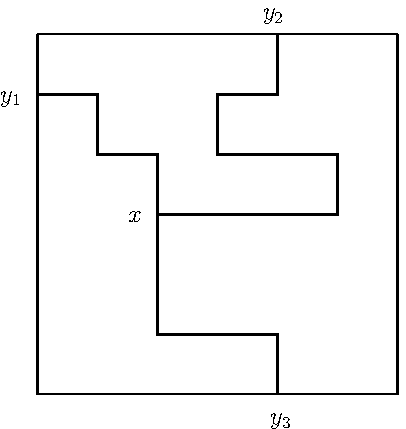
\includegraphics{pte}
\caption{O evento $\fln(\y)$.}
\eef

Logo 
\beqnn
&&\p(\fnu(\y)\cap\fln(\y))\\ \=\p(\fnu(\y))\p(\fln(\y))>0,
\eeqnn 
onde a
igualdade segue da independência dos eventos (o primeiro depende 
apenas de elos exteriores a $\qnu$; o segundo, apenas de elos interiores).

Vamos dizer agora que um ponto triplo (segundo a definição no exercício acima)
é um {\em ponto triplo especial} se seus ramos são infinitos.
Note que
$$
\{\mbox{$x(\y)$ é um ponto triplo especial}\}\supset\fnu(\y)\cap\fln(\y).
$$
De toda discussão acima, concluimos que, se $\p(\eta\geq3)>0$,
então
\beq
\p(\mbox{$x$ é um ponto triplo especial})>0.
\eeq
A probabilidade acima não depende de $x$, pela invariância por translação
de $\p$. Vamos denotá-la por $\rho$.
Segue-se que
\beq
\ep(\mbox{\#\{pontos triplos especiais em $\qnm$}\})=(2n-1)^d\rho,
\eeq
logo
\beq
\label{eq:con}
\p[\mbox{\#(pontos triplos especiais em $\qnm$})\geq(2n-1)^d\rho)]>0
\eeq
para todo $n$ (pois, para toda variável aleatória integrável X, 
$$P(X\geq E(X))>0).$$

Por outro lado, é uma conseqüência do exercício acima que o número de pontos
triplos especiais em $\qnm$ é inferior a $2d(2n-1)^{d-1}$ para toda
configuração de $\Om$ e todo $n$, o que contradiz 
(\ref{eq:con}) para $n$ suficientemente grande. 
Da contradição segue o resultado.

Vamos agora argumentar a afirmação no começo do parágrafo anterior.
Cada ramo de cada ponto triplo especial (pte) toca um (ou mais) sítios
em alguma face de $\partial\qn$ ($2d(2n-1)^{d-1}$ é o total de  
sítios em $\partial\qn$).

Considere os componentes conexos dos pte's usando apenas elos no interior
de $\qn$. Digamos que cada componente contenha $n_1,n_2,\ldots$ pte's
cada (isto é, o $i$-ésimo componente contem $n_i$ pte's). Logo
\beq
n_1+n_2+\ldots
\eeq
dá o total de pte's em $\qnm$.
Usando a linguagem do exercício acima, cada componente contem $n_i$ pontos
triplos. Daquele resultado sabemos que podemos achar pelo menos $n_i+2$
ramos distintos dentre as $3n_i$ possibilidades. Portanto, podemos achar
\beq
(n_1+2)+(n_2+2)+\ldots
\eeq 
ramos distintos de todos os pontos triplos. Como cada um toca pelo menos
um ponto das faces de $\qn$, será necessário que
\beq
n_1+n_2+\ldots\leq(n_1+2)+(n_2+2)+\ldots\leq2d(2n-1)^{d-1},
\eeq
como queríamos mostrar. $\bo$

\vspace{.5cm}

A seguir, apresentamos alguns corolários do Teorema~\ref{teo:uni}.
Lembramos que $\tau_p(x,y)$ é a função de conectividade dos sítios
$x$ e $y$, isto é,
$$\tau_p(x,y)=\p(x\leftrightarrow y).$$

\vs

\bco
\beq
\tau_p(x,y)\geq[\tep]^2
\eeq
\eco

\vs

O resultado acima tem como conseqüência que, na fase supercrítica,
a função de conectividade entre
dois pontos não decai quando a distância entre eles cresce.

\vs

\noindent {\bf Prova}

\beqnn
\tau_p(x,y)\ge\p(\mbox{$x$ e $y$ estão no mesmo aglomerado infinito})\\
\=\p(|C_x|=|C_y|=\infty)\geq\p(|C_x|=\infty)\p(|C_y|=\infty)=\tep^2,
\eeqnn
onde a primeira igualdade deve-se ao Teorema~\ref{teo:uni} e a última
desigualdade é FKG. $\bo$
\bco
$\tep$ é contínua à esquerda em $(p_c,1]$.
\eco

\noindent {\bf Prova}

Vamos construir modelos de percolação para todo $p\in[0,1]$ acoplados
usando uma família de variáveis i.i.d. Uniformes em $[0,1]$ 
$\{Z_e, e\in\ed\}$ declarando um elo $e$ $p$-aberto se $Z_e<p$
(como na prova da monotonicidade de $\tep$). Seja $C_p$ o aglomerado 
da origem com elos $p$-abertos.

Se $\pi\leq p$ então $\cpi\subset\cp$ e
\beqnn
\lim_{\pi\ua p}\tepi\=\lim_{\pi\ua p}\pp(|\cpi|=\infty)\\
\=\pp(\cup_{\pi<p}\{|\cpi|=\infty\}).
\eeqnn

Queremos mostrar que a última probabilidade acima vale $\tep$.
Consideremos então
\beq
\tep-\pp(\cup_{\pi<p}\{|\cpi|=\infty\})=\pp(|\cp|=\infty,|\cpi|<\infty\,
\forall\,\pi<p)
\eeq
para $p>p_c$. 
Para concluirmos que a última expressão é nula, basta argumentarmos que 
se $|\cp|=\infty$ e o aglomerado infinito $p$-aberto for único, então
$|\cpi|=\infty$ para algum $\pi<p$. 

De fato, nestas condições, tome $\a$ satisfazendo $p_c<\a<p$. Então,
quase certamente existe um aglomerado infinito $\a$-aberto, $\ia$, que
precisa satisfazer $\ia\sub\cp$ (pois do contrário haveria dois aglomerados
infinitos de elos $p$-abertos!). 

Logo, existe um caminho finito de elos $p$-abertos $\ga$ ligando a origem a
$\ia$. Como $\ga$ é finito e cada elo $e$ nele tem $Z_e<p$, então
$$\mu=\max\{Z_e,\,e\in\ga\}<p.$$ Se $\pi$ for tal que
$\pi\geq\a$ e $\mu<\pi<p$, então $\ia$ e $\ga$ são $\pi$-abertos.
Portanto $|\cpi|=\infty$.$\bo$

\vspace{.5cm}

O resultado acima, junto com o seguinte (que não é corolário da unicidade do
aglomerado infinito) nos diz que $\tep$ é contínua em $(\pce,1]$.

\bpro
\label{pro:cond}
$\tep$ é contínua à direita.
\epro

\vs

\noindent {\bf Prova}

Seja $A_n$ o evento de que a origem está ligada à fronteira de $\sn$ por um
caminho aberto. $(A_n)_{n\geq1}$ é uma seqüência decrescente e
$$\p(A_n)\downarrow\tep$$quando $n\uparrow\infty$. $\p(A_n)$ é contínua em $p$
(pois é um polinômio) e,
usando o modelo padrão do Capítulo 1, é fácil ver também que é crescente nesta
variável. Logo, $\tep$ é o limite decrescente de funções contínuas crescentes.
Um resultado de análise sobre funções semi-contínuas inferiores (ou um
argumento direto) nos dá o resultado. $\bo$

\bob
Como conseqüência dos dois últimos resultados, temos que $\tep$ será contínua
em $[0,1]$ se e somente se $\tepc=0$.
\eob

\vs

Para o próximo corolário, vamos dizer que ocorre um {\em cruzamento da esquerda para
a direita} no cubo $Q_n$ se houver um caminho de elos abertos contidos em $Q_n$
ligando a face esquerda de $Q_n$ a sua face direita. Denotemos por $\den$ o
evento de que tal cruzamento ocorre. $\den$ poderia ser visto como uma versão
a volume finito do evento de que há percolação. É uma decorrência do decaimento
exponencial do raio de $C$ na fase subcrítica que $\p(\den)\to0$ quando $n\to\infty$
neste caso (verifique). O caso supercrítico será tratado no próximo resultado.

\vs

\bco 
\label{cor:lrc}
Se $\tep>0$, então 
\beq
\p(\den)\to1
\eeq
quando $n\to\infty$.
\eco

\vs

Veremos no próximo capítulo que em $p=\pce$ um evento similar a $\den$
tem probabilidade que não converge
nem para 0 nem para 1 quando $n\to\infty$.

\vs

\noindent {\bf Prova}

Seja $I_m$ o evento de que algum sítio de $Q_m$ está num aglomerado infinito.
Dado $\eps>0$, escolha $m$ grande o suficiente para que 
\beq
\label{eq:lr1}
\p(I_m)>1-\eps
\eeq
(isto é possível pela discussão nos primeiros parágrafos do capítulo).

Temos que, para $n\geq m$
\beq
I_m\subset\cup_{i=1}^{2d}\left\{Q_m\lr F_i\,\mbox{em}\, Q_n\right\},
\eeq
onde $F_1,\ldots,F_{2d}$ são as faces de $Q_n$.

Logo
\beqn
\nonumber
1-\p(I_m)\ge1-\p\left(\cup_{i=1}^{2d}\left\{Q_m\lr F_i\,\mbox{em}\,
    Q_n\right\}\right)\\
\nonumber
\=\p\left(\cap_{i=1}^{2d}\left\{Q_m\lr F_i\,\mbox{em}\,
    Q_n\right\}^c\right)\\
\label{eq:lr2}
\ge\left[1-\p\left(Q_m\lr F\,\mbox{em}\,
    Q_n\right)\right]^{2d},
\eeqn
onde $F\in\{F_1,\ldots,F_{2d}\}$ e a última desigualdade segue de 
FKG pelo fato de que os eventos
na intersecção são decrescentes e também do fato que estes eventos
têm a mesma probabilidade (vide prova do Lema~\ref{le:leb1} na 
página~\pageref{le:leb1}).

De~(\ref{eq:lr1}) e~(\ref{eq:lr2}), temos que
\beq
\label{eq:lr3}
\p\left(Q_m\lr F\,\mbox{em}\,Q_n\right)\geq 1-\eps^{1/{2d}}
\eeq

Sejam $F_e$ e $F_d$ as faces esquerda e direita de $Q_n$ respectivamente.
Por FKG e~(\ref{eq:lr3}),
\beq
\p\left(\{Q_m\lr F_e\,\mbox{em}\,Q_n\}\cap\{Q_m\lr
  F_d\,\mbox{em}\,Q_n\}\right) \geq (1-\eps^{1/{2d}})^2
\eeq

Seja agora $\amn$ o evento de que há 2 sítios em $\del Q_m$ em 2 aglomerados
abertos disjuntos, ambos tocando $\del Q_n$. Temos que $\amn\supset\amnu$ e
$\amn\downarrow A_m$ quando $n\uparrow\infty$, onde $A_m$ é o evento de que
há 2 aglomerados abertos infinitos disjuntos tocando $Q_m$.

\bef
%\input amn
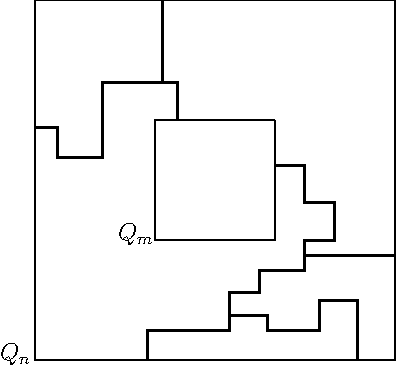
\includegraphics{amn}
\caption{O evento $\amn$}
\eef

Em conclusão
\beq
\p(\amn)\to\p(A_m)=0
\eeq
quando $n\to\infty$ e portanto, de
\beq
\p(\den)\geq (1-\eps^{1/{2d}})^2-\p(\amn),
\eeq
que decorre de
\beq
\{Q_m\lr F_e\,\mbox{em}\,Q_n\}\cap\{Q_m\lr
  F_d\,\mbox{em}\,Q_n\}\subset\den\cup\amn,
\eeq
temos
\beq
\liminf_{n\to\infty}\p(\den)\geq (1-\eps^{1/{2d}})^2
\eeq
e o resultado segue de $\eps$ ser arbitrário. $\bo$
















